\documentclass[]{article}
%\usepackage[margin=1in]{geometry}
%\usepackage{setspace}
\usepackage{natbib}
\usepackage{pdfpages}
\usepackage[euler]{textgreek}
\title{The Runner's High}
\author{Nakul Joshi}
\date{April 15, 2013}
%\doublespacing
\begin{document}
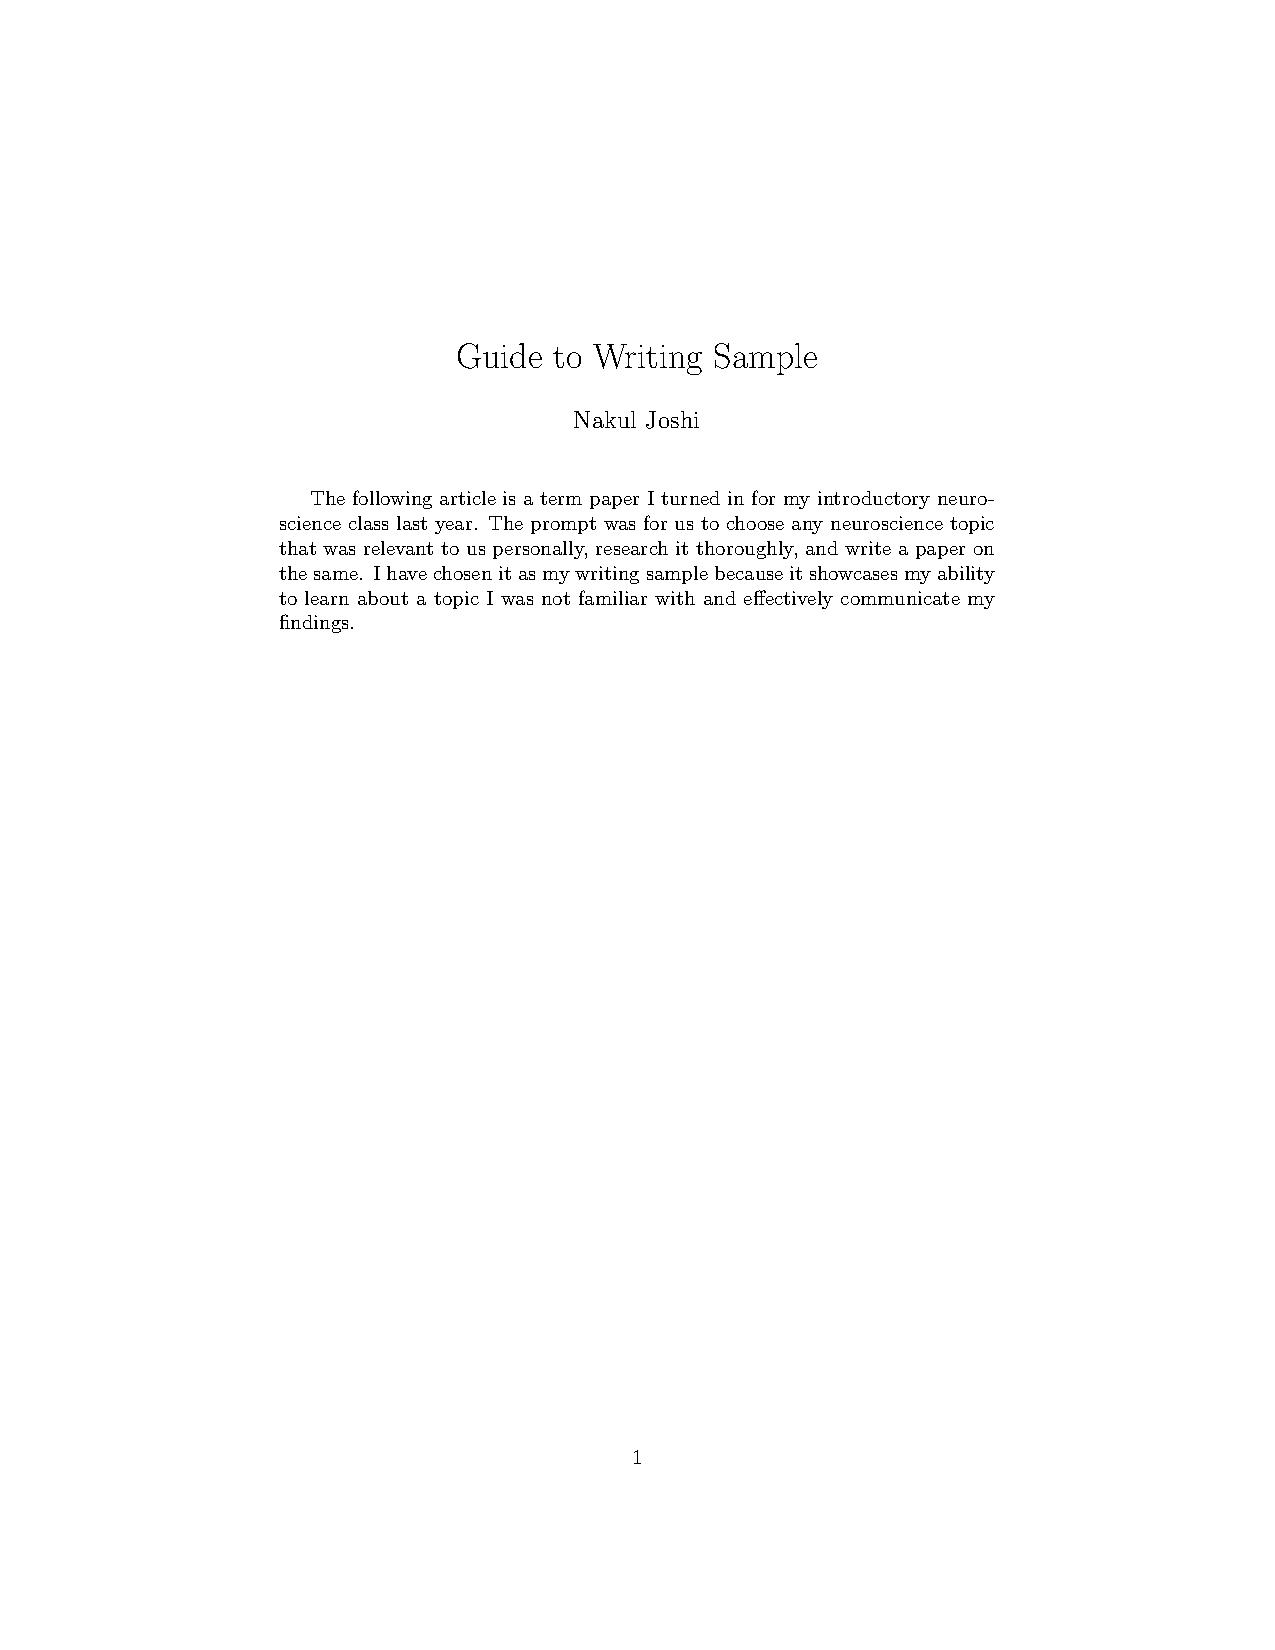
\includepdf{guide.pdf}
\maketitle

\paragraph{Abstract} \textit{A large portion of the running community subscribes to a belief in the concept of the so-called `runner's high'. In this paper, I will describe the scientific evidence for and against the existence of the phenomenon, and examine the mechanisms that might explain its causes and effects. I will compare the conclusions of research with my own experiences with running, and will also examine the potential consequences that such a phenomenon might have for runners and athletes in general.}

\section{Introduction}

	Until recently, I have been a very inactive person, usually confined to a work-desk, couch, or a kitchen table. Thus, whenever I watched marathons or other endurance sports, I was very surprised by the capacity of some human beings to continue performing a strenuous task for hours on end, and often wondered what allowed them to overcome the pain it must cause them. Thinking that they were simply born with an immunity to exhaustion that I did not posses, I stayed well away from such sports.
	
	This changed when, a few years ago, I befriended a triathlete. When I asked him what allowed him to run miles on end right after swimming in frigid water, he told me of the `high' he got after any extended period of physical activity. I initially dismissed this as just another strange belief of triathletes, who already seemed like a cult in my mind. However, he encouraged me to try doing some running of my own, and I was intrigued enough to do so. At first, the runs were painful to my feet, harsh on my lungs, and almost always left me feeling nauseous. As I began running longer and longer distances though, I noticed that I began enjoying the exertion. I ended my laps feeling euphoric rather than drained, and I encountered my first few experiences of the runner's high. However, these incidents were sporadic in occurrence, and it remained difficult to tell if they corresponded to real, physical changes to my body, or merely to suggestions that had been supplied to my imagination.

\section{Is it real?}

	Besides sundry tales from various athletes, there has, until fairly recently, been little qualitative and objective study of the runner's high phenomenon. Research suggests \citep{mood, mood2} that exercise is correlated with a general reduction in anxiety and depression. These conclusions are matched by experimentation on rodents, which show that exercise can increase pain tolerance and have a sedative action \citep{endocan,ratrun}. However, it is unclear whether these general effects are the same as the specific phenomenon that runners call the `high'.
	
	This suggests that the biggest difficulty with verifying the existence of the high is that there is no good description of what it actually is. Popular descriptions vary from `pleasantness' to `a feeling of inner peace'. In order to define the `high' in a manner that is compatible with testable hypotheses, it has been suggested \citep{endocan} that the high be parametrised by ``observable behaviours such as analgesia, sedation (post-exercise calm) , anxiolysis, and a sense of wellbeing". Operating under definitions like these, research shows a strong validation of the legitimacy of the phenomenon \citep{endocan, opioid}. My own few experiences with the high seemed correlated with these parameters, and this led me to wonder how it worked.
	
\section{Mechanism of action}
	Almost everybody is aware of the `pop culture' explanation of the high- it seems almost common knowledge that exercise causes a release of endorphins, which in turn cause a release of dopamine, which interact with the nucleus accumbens (commonly called the `pleasure' or `reward' centre of the brain) to cause a feeling of euphoria, in a manner similar to the action of recreational drugs.
	
	However, this mechanism has been criticised as being overly simplistic and inaccurate, without enough scientific evidence to raise it beyond the level of myth or urban legend \citep{fiction}. Modern work has greatly improved from this starting point, and I shall now present three of the prevailing theories behind the high.
	
	\subsection{The Opioid Theory}	
	Opioids are a class of psychoactive compounds that bind to opioid receptors in the nervous system. Their effects on the body have been known and exploited by societies from before recorded history, who used them medically (as painkillers) as well as recreationally, commonly extracting them as opium from the poppy. They are a wide class of drugs, encompassing morphine, codeine, and heroin. The term `endorphin' (endogenous morphine) derives its name from the fact that it is used to describe opioid (morphine-like) compounds that are supposedly produced within the body itself (`endo-') during exercise.

	Work by \citep{endorphin} provided early evidence for this hypothesis, however it was based on measurement of endorphins in the circulating blood, and it has been questioned \citep{endocan} whether this corresponds to any psychological changes, because \textbeta -endorphins are considered too big to pass through the blood-brain barrier in significant amounts. Further research into this hypothesis has long been inhibited by the infeasibility of performing lumbar punctures (`spinal taps') on athletes before and after exercise, to measure endorphin levels in the cerebrospinal fluid \citep{overview}.
	
	However, advancements in technology allowed one group \citep{opioid} to indirectly measure these endorphins via PET (positron emission tomography) scannning. Their data supports the opioid hypothesis, while specifically identifying sites of the brain (the frontolimbic areas) that mediated this action. Another group showed that the painkilling action of exercise on rats was mediated by their opioid receptors \citep{ratrun}.
	
	\subsection{The Endocannabinoid Theory}
	
	Cannabinoids are another class of psychoactive compounds, and these activate cannabinoid receptors. They serve as retrograde transmitters, signalling opposite to the direction of the synapses. Cannabinoids are the priamary active ingredient in cannabis or marijuana, and cause effects of relaxation and a heightened awareness of sensation.
	It has been shown that these effects can be replicated by exercise \citep{endocan}, and that the cannabinoid mechanism of analgesic action is consistent with the observations of exercise induced analgesia. Further, it has also been shown that there is a connection between the addictive natures of both cannabis and long distance running \citep{endocan}.
	
	However, the authors of this paper strongly emphasise that more research into the specific mechanisms of action of cannabinoids is needed before much can be said about any particulars of cannabinoid response, or the weights of factors such as exercise duration and intensity, nature of the activity, or characteristics of the individual. 
	
	\subsection{The Placebo Effect}
		Finally, it might just be that the primary mechanism of the runner's high is the placebo effect; in other words, it is merely the \emph{expectation} of euphoria and pain relief that cause the same effects. It has been argued \citep{placebo} that just as placebos have been demonstrated to cause pain relief as well as a rise in endorphin secretion in subjects who were told to expect such effects, runners might feel euphoria because popular culture makes them expect it.		
		
\section{Why the high?}
	Perhaps it would be more instructive, and more interesting, to ask why, as opposed to how, the runner's high occurs.
	
	It has been suggested \citep{hunt} that humans have evolved as persistance hunters, tracking and following prey over long distances until they have been exhausted.This would have allowed early humans to catch animals that would otherwise easily outrace them. As one of the few creatures with an effective sweat-based thermeoregulation system to keep them cool, humans would have had a significant advantage over other animals in long-distance runs. Perhaps the high evolved as a mechanism to cope with the pain and injuries that long distance running causes.
	
	Another proposed explanation for the high is the activation of the reward centres of the brain that is associated with any goal-fulfilling activity. It has been shown \citep{happiness} that keeping track of one's progress of improvement at any task is an excellent motivator to keep at practicing, and that training at new skills is an important contributor to feelings of happiness.
	
	Reading over Haidt's arguments, I remembered that my own highs were the most exhilarating  when I noticed the long-term improvement of my running pace. Seeing myself go from panting after running one mile in seventeen minutes to finishing two miles in the same time and not even feeling tired has been one of the most exciting and happy moments of my life- it wasn't just the physical activity that made me happy, but also the knowledge of how much I had improved, and of how much better the quality of my life was as I became more fit.
	
\section{Conclusions}

	While most research agrees with the existence of the runner's high, there is still some disagreement on what exactly the phenomenon \emph{is}. The personal nature of this experience, along with it's intermittent occurence and high variability, makes it hard to describe in any meaningful manner, and perhaps this represents a fundamental limit to how well we can quantise this effect.
	
	More research is clearly needed to explain the mechanisms behind the high- there are several competing theories, and it would be na\"{\i}ve to think that only one or two types of compounds are involved in mediating the psychological responses to exercise. If the runner's high is a complex interaction within a system composed of several types of neurotransmitters, and mediated by different parts of the brain in different ways, it will be incredibly difficult to uncover the entire mechanism of response.
	
	Regardless, the nature of the high is clearly beneficial as a motivator for physical activity- the promise of that feeling helps me get out of bed early for a run when I would rather snooze, and the detachment generated has helped me make it through that last stretch when I would otherwise be stopped by pain. It offers one of the few healthy alternatives to the typical avenues of stress relief such as alcohol and nicotine, strengthening and maintaining the body rather than damaging it.

\bibliographystyle{plainnat}
\bibliography{bisc230}
\end{document}